\section{Experimental Evaluation}
\label{sec:exp}

\begin{figure*}[t]
\vspace{-0.2in}
\centering
\begin{minipage}[b]{2.1in}
\centering
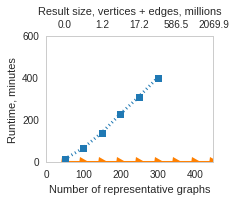
\includegraphics[width=2.1in]{figs/slice_ngrams_build13.png}
\vspace{-0.2in}
\caption{Slice on nGrams.}
\label{fig:slicengrams}
\vspace{-0.1in}
\end{minipage}
\begin{minipage}[b]{2.1in}
\centering
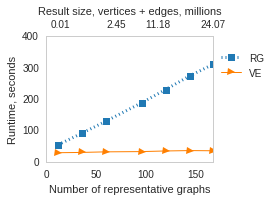
\includegraphics[width=2.1in]{figs/project_wikitalk_build13.png}
\vspace{-0.2in}
\caption{Map on wiki-talk.}
\label{fig:project}
\vspace{-0.1in}
\end{minipage}
\begin{minipage}[b]{2.2in}
\centering
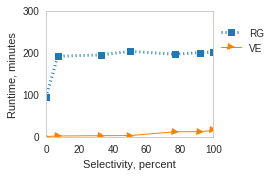
\includegraphics[width=2.4in]{figs/subgraph_ngrams_build13.png}
\vspace{-0.2in}
\caption{Subgraph on nGrams.}
\label{fig:subgraphngrams}
\vspace{-0.1in}
\end{minipage}
\end{figure*}

\begin{figure*}[t!]
\centering
\begin{subfigure}{0.3\textwidth}
%\begin{minipage}{2.2in}
%\centering
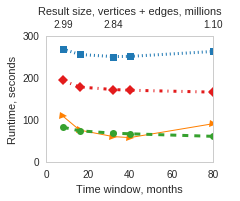
\includegraphics[width=2.2in]{figs/agg_allall_wikitalk_build13.png}
\caption{$q_v=\insql{always}$, $q_e=\insql{always}$, wiki-talk}
\label{fig:agg1}
%\end{minipage}
\end{subfigure}
\begin{subfigure}{0.3\textwidth}
%\begin{minipage}{2.2in}
%\centering
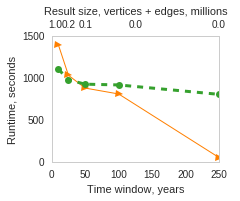
\includegraphics[width=2.2in]{figs/agg_allexists_ngrams_build13.png}
\caption{$q_v=\insql{always}$, $q_e=\insql{exists}$, nGrams}
\label{fig:agg2}
%\end{minipage}
\end{subfigure}
\begin{subfigure}{0.36\textwidth}
%\begin{minipage}{2.5in}
%\centering
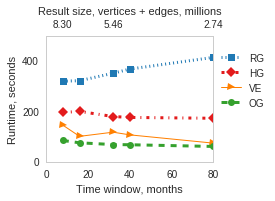
\includegraphics[width=2.5in]{figs/agg_allexists_wikitalk_build13.png}
\caption{$q_v=\insql{always}$, $q_e=\insql{exists}$, wiki-talk}
\label{fig:agg4}
%\end{minipage}
\end{subfigure}
\vspace{-0.1in}
\caption[]{Node creation with temporal windows.}
\vspace{-0.1in}
\label{fig:agg}
\end{figure*}

\subsection{Setup}
\label{sec:exp:setup}

All experiments were conducted on a 16-slave in-house Open Stack
cloud, using Linux Ubuntu 14.04 and Spark v2.0.  Each node has 4 cores
and 16 GB of RAM.  Spark Standalone cluster manager and Hadoop 2.6
were used.
%
Because Spark is a lazy evaluation system, a materialize operation was
appended to the end of each query, which consisted of the count of
nodes and edges.  Each experiment was conducted 3 times with a cold
start -- the running time includes the setup time of submitting the
job to the cluster manager, uploading the jar to the cluster, reading
the data from disk, building the chosen representation, and running
a single query.  We report the average running time, which is
representative because we took great care to control variability:
standard deviation for each measure is at or below 5\% of the mean
except in cases of very small running times.  No computation results
were shared between subsequent runs.

\eat{OG and HG inherit their implementation of \insql{slice}, \insql{map}
and \insql{subgraph} from RG and are not included in these
experiments.  Performance of all 4 data structures is compared in
\insql{aggregation}, \insql{union} and \insql{intersection}.}

{\bf Data.}  We evaluate performance of our framework on three real
open-source datasets, summarized in Table~\ref{tab:datasets}.
wiki-talk (\url{http://dx.doi.org/10.5281/zenodo.49561}) contains over
10 million messaging events among 3 million wiki-en users\eat{2002
  through 2015}, aggregated at 1-month resolution.\\nGrams
(\url{http://storage.googleapis.com/books/ngrams/books/datasetsv2.html})
contains word co-occurrence pairs\eat{ from 1520 through 2008}, with
30 million word nodes and over 2.5 billion undirected edges.  The
Twitter social graph~\cite{Gabielkov:2014:SSN:2591971.2591985}
contains over 23 billion directed follower relationships between 0.5
billion twitter users\eat{ collected in 2012}, sampled at 1-month
resolution.\eat{ based on account creation information from April
  2006.} \eat{DELIS contains monthly snapshots of a portion of the Web
  graph focusing on the .uk domains from 05/2006 through
  05/2007~\cite{BSVLTAG}. }The datasets differ in size, in the number
and type of attributes and in evolution rates, calculated as the
average graph edit similarity~\cite{Ren2011}. \eat{the evolutionary
  properties: co-authorship network nodes and edges have limited
  lifespan, while the nGrams network grows over time, with nodes and
  edges persisting for long duration.  All figures in the body of this
  section are on the larger nGrams dataset.  Refer to the Appendix for
  the DBLP figures, which show similar trends as nGrams.}

\eat{The behavior of the four physical representations reported below is
dependent on the underlying data format on disk
(Section~\ref{sec:sys:maint}), and should be interpreted in that
context.}

\subsection{Individual operators}
\label{sec:exp:ops}

{\bf Slice} performance was evaluated by varying the slice time window
and materializing the \tg, and is presented in
Figures~\ref{fig:slicengrams} for nGrams and~\ref{fig:slicewiki} for
wiki-talk (in Appendix~\ref{sec:app2}).  Similar trends were observed
for twitter.  Slice is expected to be more efficient when executed
over VE when data is coalesced on disk than over \sg, and we observe
this in our experiments.  This is because multiple passes over the
data are required for \sg to compute each representative graph,
leading to linear growth in running times for file formats and systems
without filter pushdown, as is the case here.  Slice over VE simply
executes temporal selection and has constant running times (29 sec for
wiki-talk, about 1.5 min for nGrams).\eat{Recall that in VE
  \insql{slice} performs temporal selection, and method when data on
  disk is coalesced.  \sg, in contrast, does multiple passes of select
  over the same data to compute each RG.  Thus, as expected, VE
  behavior is directly dependent on the size of input data regardless
  of the slice size for file formats and systems without filter
  pushdown, as is the case here, or if the data does not have temporal
  locality (Figure~\ref{fig:slicewiki}, Figure~\ref{fig:slicengrams}
  -- about 1.5 minutes for VE).  \sg behavior is linear in the slice
  size. } This experiment essentially measures the cost of
materializing \sg from its on-disk representation. \eat{ We observed the
same linear trend in our preliminary work, when the data was stored as
individual snapshots on disk, although less redundant work is needed
in that case.}

{\bf Vertex subgraph} performance was evaluated by specifying a
condition on the $length(a.attr)<t$ of the vertex attribute, with
different values of $t$ leading to different selectivity.  This
experiment was executed for wiki-talk (with $username$ as the
property) and for nGrams (with $word$ as the property).  Twitter has
no vertex attributes and was not used in this experiment.
Figure~\ref{fig:subgraphngrams} shows performance for \sg and VE on
nGrams (wiki-talk results in Appendix~\ref{sec:app2}).  Performance on
\sg is a function of the number of intervals and is insensitive to the
selectivity.  The behavior on VE is dominated by FK enforcement:
with high selectivity (few vertices) broadcast join affords
performance linear in the number of edges, whereas for a large number
of vertices broadcast join is infeasible and a hash-join is used
instead, which is substantially slower.  VE provides an order of
magnitude better performance than \sg: up to 3 min with hash-join and
up to 15 min with broadcast join for VE, in contrast to between 95 and
200 min for \sg.

{\bf Map}\eat{ We evaluate \insql{map} performance by varying the data
  size through the \insql{slice} operation.} exhibits a similar trend
as \insql{slice}: constant running time for VE and a linear increase
in running time with increasing number of representative graphs for
\sg (Figure~\ref{fig:project} for wiki-talk, similar for other
datasets).  Performance of \insql{map} is slightly worse than that of
\insql{slice} because \insql{map} must coalesce its output as the last
step, while \insql{slice} does not. 

\begin{table}
\caption{Experimental datasets.}
\vspace{-0.1in}
\small
\begin{tabular}{l | c | c | c | c }
\hline
\multicolumn{1}{l|}{\bfseries Dataset} & \multicolumn{1}{c|}{\bfseries |V|} & \multicolumn{1}{c|}{\bfseries |E|} & \multicolumn{1}{c|}{\bfseries Time Span} & \multicolumn{1}{c}{\bfseries Evol. Rate} \\ \hline
wiki-talk-en & 2.9M & 10.7M & 2002--2015 & 14.4 \\ \hline
nGrams & 29.3M & 2.5B & 1520--2008 & 16.67 \\ \hline
%%DELIS & 128M & 40.5B & 2006--2007 & ? \\ \hline
twitter & 505.4M & 23B & 2006--2012 & 88 \\ \hline
\end{tabular}
\vspace{-0.1cm}
\label{tab:datasets}
\end{table}

\begin{figure*}[t]
\begin{minipage}{2.1in}
\centering
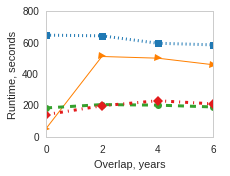
\includegraphics[width=2.1in]{figs/union_wikitalk_build13.png}
\vspace{-0.2in}
\caption{Union on wiki-talk.}
\label{fig:union1}
\vspace{-0.1in}
\end{minipage}
\begin{minipage}{2.1in}
\centering
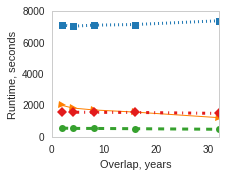
\includegraphics[width=2.1in]{figs/union_ngrams_build13.png}
\vspace{-0.2in}
\caption{Union on nGrams.}
\label{fig:union2}
\vspace{-0.1in}
\end{minipage}
\begin{minipage}{2.2in}
\centering
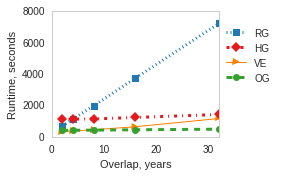
\includegraphics[width=2.55in]{figs/intersect_ngrams_build13.png}
\vspace{-0.2in}
\caption{Intersection on nGrams.}
\label{fig:intersectngrams}
\vspace{-0.1in}
\end{minipage}
\end{figure*}

\begin{figure*}[t]
\centering
\begin{minipage}{2.15in}
\centering
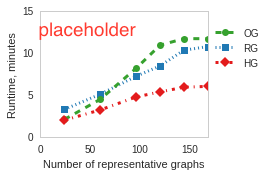
\includegraphics[width=2.15in]{figs/deg_twitter_build14.png}
\vspace{-0.2in}
\caption{Aggregate on Twitter.}
\label{fig:degtwitter}
\vspace{-0.1in}
\end{minipage}
\begin{minipage}{2.15in}
\centering
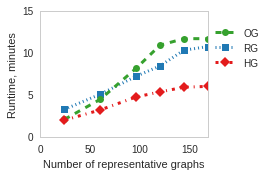
\includegraphics[width=2.15in]{figs/cc_wikitalk_build13.png}
\vspace{-0.2in}
\caption{Components on wiki-talk.}
\label{fig:ccwiki}
\vspace{-0.1in}
\end{minipage}
\begin{minipage}{2.2in}
\centering
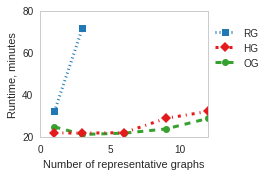
\includegraphics[width=2.2in]{figs/prank_twitter_build13.png}
\vspace{-0.2in}
\caption{PageRank on Twitter.}
\label{fig:pranktwitter}
\vspace{-0.1in}
\end{minipage}
\end{figure*}

{\bf Aggregation} performance was evaluated on the graph-based
representations with a computation of vertex degrees, varying the size
of the temporal window obtained with slice.  The results in
Figure~\ref{fig:degtwitter} indicate that materialization of each
representative graph required for \sg makes it not a viable candidate
for this operation, especially over large datasets.  Both \og and \hg
exhibit linear increase in performance as the slice size is increased,
with a small slope.  Similar performance was observed in the other
datasets.

{\bf Node creation} performance was evaluated on all representations,
since all have different implementations of this operator.  We
executed topology-only creation (no attributes), varying the size
of the temporal window.  We observe that performance depends heavily
on the quantification, and on the data evolution rate.  \og is an
aggregated data structure with good temporal locality and thus in most
cases provides good performance and is insensitive to the temporal
window size (Figure~\ref{fig:agg1}).  However, in datasets with a
large number of representative graphs (such as nGrams), \og is slow on
large windows, an order of magnitude worse than VE in the worst case
(Figure~\ref{fig:agg2}).  VE outperforms \og when vertex and edge
quantification levels match (Figure~\ref{fig:agg1}), but is worse than
\og when vertex quantification is stricter than edge quantification
and FK must be enforced (Figure~\ref{fig:agg4}).  \og also outperforms
VE when both evolution rate is low and aggregation window is small
(Figure~\ref{fig:agg1}, wiki-talk).\eat{ \sg and \hg do not provide
  the best performance on any of our datasets.}

{\bf Union, intersection, and difference} by structure were evaluated
by loading two time slices of the same dataset with varying temporal
overlap.  Performance depends on the size of the overlap (in the
number of representative graphs) and on the evolution rate.  VE has
best performance when overlap is small (Figure~\ref{fig:union1})\eat{
  and when the evolution rate is high (Figure~\ref{fig:union2}),
  regardless of the size of the overlap}.  \og always has good
performance, constant w.r.t. overlap size.  This is expected, since
\og \insql{union} and \insql{intersection} are implemented as joins
(outer or inner) on the vertices and edges of the two operands.  VE,
on the other hand, splits the coalesced vertices/edges of each of the
two operands into intervals first, takes a union, and then reduces by
key.  When evolution rate is low and duration of an entity is high,
such as in wiki-talk for vertices, the split produces a lot of tuples
to then reduce, and performance suffers (Figure~\ref{fig:union1}). \sg
only has good performance on \insql{intersection} when few
representative graphs overlap, and never on \insql{union}
(Figure~\ref{fig:intersectngrams}). \hg performance is worse than \og,
by a constant amount in \insql{union}, and diverges in
\insql{intersection}.  \eat{\insql{difference} performance is similar
  to \insql{intersection}.}

{\bf Analytics.}  We implemented PageRank (PR) and Connected
Components (CC) analytics for the three graph-based representations
using the Pregel GraphX API.  PR was executed for 10 iterations or
until convergence, whichever came first. CC was executed until
convergence with no limit on the number of iterations.  Performance of
Pregel-based algorithms depends heavily on the partitioning strategy,
with best results achieved where cross-partition communication is
small~\cite{MoffittTempWeb16}.  For this reason, we evaluated only
with the E2D strategy.
%
Performance was evaluated on time slices of varying size.  Recollect
that analytics are essentially multiple rounds of aggregate
operations, so the performance we observe is an amplified version of
aggregate performance.  For a very small number of graphs (1-2), \sg
provides good performance, but slows down linearly as the number of
graphs increases.  \hg provides the best performance on analytics
under most conditions, with a linear increase but a significantly
slower rate of growth.  The tradeoff between \og and \hg depends on
graph evolution characteristics.  If the graph is a growth-only
evolution (such as in Twitter), \og is not denser than \hg and
computes everything in a single batch, which leads to the fastest
performance, as can be seen in Figure~\ref{fig:pranktwitter}.  If the
edge evolution represents more transient connections, then \hg is less
dense and scales better (Figure~\ref{fig:ccwiki}).  Note that \og and
\hg performance could be further improved by computing them over
coalesced structure-only V and E, and ignoring attributes.

{\bf In summary,} no one data structure is most efficient across all
operations.  This opens the door to query optimization based on the
characteristics of the data such as graph evolution rate and on the
type of operation being performed.  

\eat{VE provides the best
  performance for slice, map, and subgraph.  \og is efficient for
  aggregation under most conditions, and \hg for analytics.  The graph
  evolution rate is an important factor in selecting the more suitable
  representation.}

\subsection{Switching between representations}
\label{sec:exp:scale}

\begin{figure*}[t]
\centering
\begin{minipage}{2.2in}
\centering
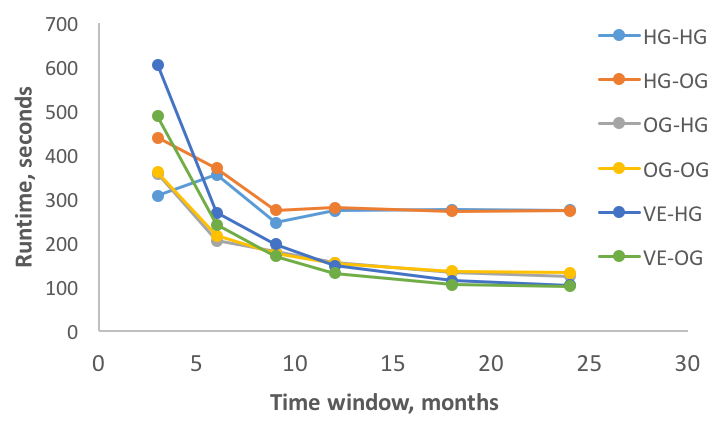
\includegraphics[width=2.1in]{figs/switch_cc.png}
%\vspace{-0.2in}
\caption{$\insql{node}^T_a$ followed by components.}
\label{fig:ncrtocc}
\vspace{-0.1in}
\end{minipage}
\begin{minipage}{2.2in}
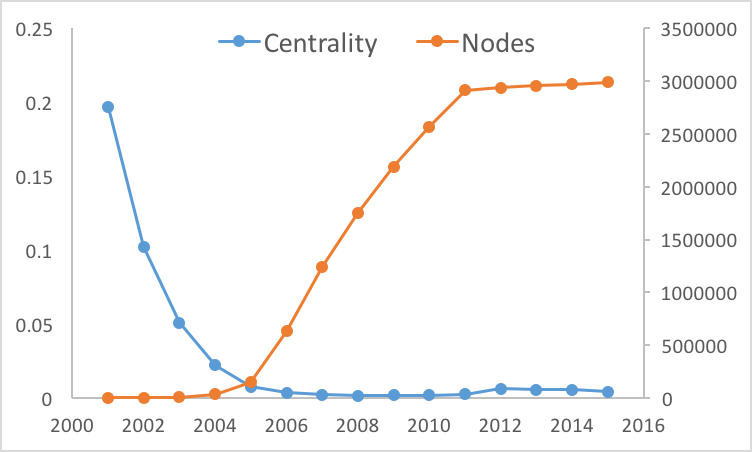
\includegraphics[width=2.2in]{figs/centrality.png}
\caption{In-degree centrality with 1 year resolution.}
\label{fig:central}
\end{minipage}
\begin{minipage}{2.2in}
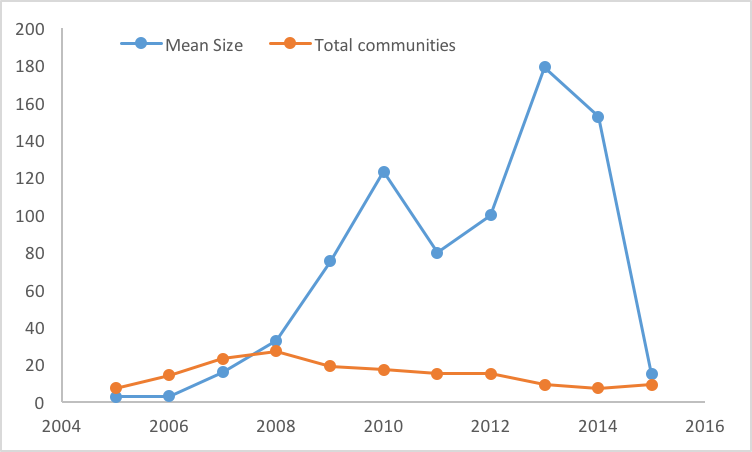
\includegraphics[width=2.2in]{figs/communities.png}
\caption{Communities with 1 year resolution.}
\label{fig:commun}
\end{minipage}
\end{figure*}

To treat the four representations as access methods, we need to be
able to switch between them.  The data structures can be created from
outputs of any of the four, at a cost.  To investigate the feasibility
of switching between representations, we executed two-operator queries
and either kept the representation constant or changed it between the
operators.  The query is based on the first two steps of example three
in our motivating use cases: node creation over temporal windows in
wiki-talk, followed by the connected components analytic.
Figure~\ref{fig:ncrtocc} shows the result of varying the size of the
temporal window.  Recall that \og is the best performing
representation for node creation at small windows and \hg for
components over this dataset.  The benefits of \hg are substantially
consumed by switching: the performance of \og-\og and and \og-\hg are
similar.  If the cost of switching was negligable, then \og-\hg should
have exhibited notably better performance than all other combinations.
However, the \og-\hg still performs best over-all, indicating that
switching is feasible.

\eat{{\bf Cluster Size.}  We next examine how the system performance scales
with the size of the cluster.  We execute
\insql{slice; aggregate(1 year, exists, exists); components}.}
%
\eat{
\begin{small}
\begin{verbatim}
   slice
   aggregate(1 year, exists, exists)
   connected components
   materialize vertices
\end{verbatim}
\end{small}
}
\eat{This query, executed on the wiki-talk dataset, computes connected
components over the past 10 years on the yearly scale.  Over the
twitter dataset the slice size is 2 years.}

%%\begin{small}
%%\begin{verbatim}
%%Q2. UKDELIS
%%
%%   aggregate(3 months, exists, always)
%%   pagerank(20 iterations)
%%   project pagerank score
%%   aggregate(12 months, exists, exists, trend)
%%   get top 10
%%\end{verbatim}
%%\end{small}
\eat{
This query, executed on DELIS dataset, computes stable links between
websites, i.e. links that persist for 3 months, and uses them to
compute pagerank for each.  The score is projected and its trend
computed in an aggregation over the whole dataset time period (1
year).  The top 10 websites with the highest increase in pagerank are
returned.
}

\eat{The best performing representation was selected based on our
experimental results.  Slice, project, and aggregate were performed
with VE, analytics with \hg.  The results are in
Table~\ref{tab:clustersize}.  Both queries show improvements in
running time as the cluster size grows, with diminishing returns.}
\eat{With the small wiki-talk dataset, performance improves initially
  with larger cluster sizes but levels off at the largest size.  With
  the large twitter dataset, ...}

\eat{
\begin{table}
\centering
\caption{Effect of cluster size, minutes.}
\vspace{-0.1in}
\small
\begin{tabular}{| l | c | c | c | c |}
\hline
\multicolumn{1}{|l|}{\bfseries Dataset} & \multicolumn{1}{c|}{\bfseries 4 slaves} & \multicolumn{1}{c|}{\bfseries 8 slaves} & \multicolumn{1}{c|}{\bfseries 12 slaves} & \multicolumn{1}{c|}{\bfseries 16 slaves}\\ \hline
wiki-talk & 8.41 & 6.02 & 5.02 & 2.94 \\ \hline
Twitter & 151.77 & 72.75 & 55.68 & 53.46 \\ \hline
\end{tabular}
\label{tab:clustersize}
\end{table}
}



\subsection{Use cases}
\label{sec:exp:cases}

To see how our algebra handles the use cases from
Section~\ref{sec:cases}, we implemented each one over the wiki-talk
dataset.  Each example requires a sequence of operators.  For each
operator we used the best performing data structures based on the
comparison experiments described above.

Example 1 answers the question of whether there are high influence
nodes and whether that behavior is persistent in time.  The code to
compute the answer is 4 lines of a Scala program and the query took 76
seconds to execute.  The results show that from 25 nodes with mean
degree of 40 and above that have persisted for at least 6 months, 6
have coefficient of variation below 50, which is quite low, and only 5
have it above 100.  This indicates that there are in fact high
in-degree nodes and that they continue to be influential over long
periods of time, despite the loose connectivity of the overall
network.

\eat{
\begin{verbatim}
    val deg = g.aggregateMessages[Int](triplet => { Iterator((triplet.dstId, 1)) }, (a, b) => {a+b}, 0, TripletFields.None).mapVertices((vid, intv, attr) => Map(intv -> attr._2), Map[Interval,Int]())
    val agg = deg.createNodes(ChangeSpec(g.getTemporalSequence.count.toInt), Exists(), Exists(), (a, b) => {a ++ b}, anyfun)()
    val unit = Resolution.from("P1M").unit
    println("lowest coefficient of variation (largest stability) top 10 users: " + agg.mapVertices((vid, intv, attr) => { val allpoints = TempGraphOps.makeSeries[Int](attr, Some(0)).map(x => x.getOrElse(0)); val mean = allpoints.sum / allpoints.size.toDouble; val variance = allpoints.map(x => math.pow(x - mean, 2)).reduce(_ + _) / allpoints.size; (mean, math.sqrt(variance) / mean * 100, allpoints.size)}, (0.0, 100.0, 1)).vertices.filter(x => x._2._2._1 > 0.0).sortBy(x => x._2._2._1, ascending = false).take(50).mkString("\n"))
\end{verbatim}
}

\eat{
\begin{figure}
\centering
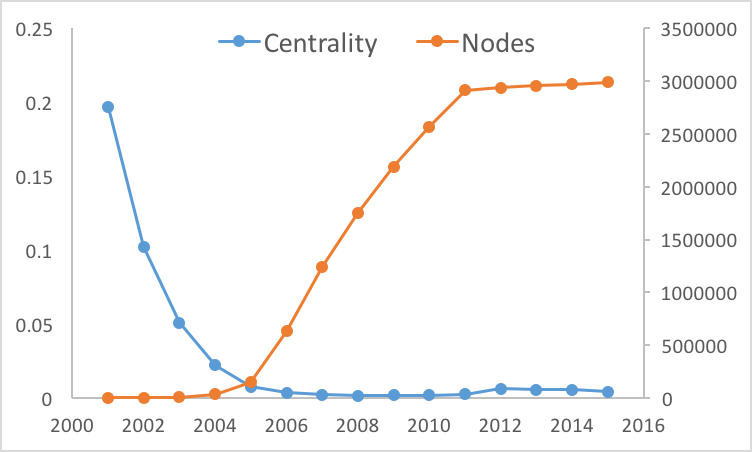
\includegraphics[width=2.2in]{figs/centrality.png}
\caption{In-degree centrality with 1 year resolution.}
\label{fig:central}
\end{figure}}

Example 2 examines how the graph centrality changes over time.  The
program is 6 lines of Scala code iterating with temporal windows of 1,
2, 3, 6, and 12 months, and the analysis took 25 minutes.  Results
show that regardless of the temporal resolution, the in-degree
centrality is extremely low, about 0.04.  Figure~\ref{fig:central}
provides an explanation -- as the size of the graph increases, its
centrality decreases.  Given that the number of edges in this graph is
only about 4 times the number of nodes, the graph is too sparse and
disjointed to have any centrality.

\eat{
\begin{table}
\centering
\caption{In-degree centrality over time in wiki-talk}
\small
\begin{tabular}{| l | c | c |}
\hline
\multicolumn{1}{|l}{\bfseries Window} & \multicolumn{1}{c|}{\bfseries Mean} & \multicolumn{1}{c|}{\bfseries StDev} \\ \hline
1 & 0.03 & 0.09 \\
2 & 0.04 & 0.11 \\
3 & 0.04 & 0.13 \\
6 & 0.06 & 0.18 \\
12 & 0.03 & 0.05 \\ \hline
\end{tabular}
\label{tab:centrality}
\end{table}
}

\eat{\begin{figure}
\centering
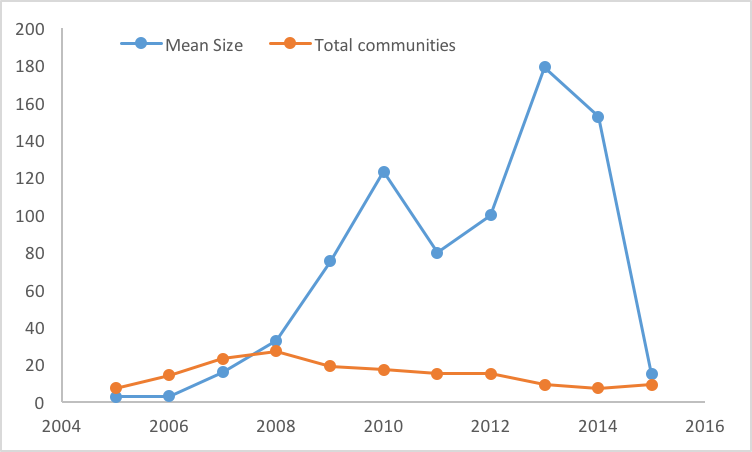
\includegraphics[width=2.2in]{figs/communities.png}
\caption{Communities with 1 year resolution.}
\label{fig:commun}
\end{figure}}

Finally, example 3 examines whether communities can be detected in the
wiki-talk network at different temporal resolution.  The program,
similar to the one above, is 6 lines of Scala code with varied
temporal windows.  The total runtime is 58 minutes.  Communities,
defined as connected components, can be detected in all temporal
resolutions.  As a reminder, the edge quantification in this query is
\insql{always}, so only edges that persist over each window are
retained.  The presence of communities even with large temporal
resolution indicates that communities form and persist over time.
Figure~\ref{fig:commun} shows the mean size of all communities by time
and their total number.  The peaks of the mean size, visible in all
temporal windows, may indicate that communities form and then reform
in a different configuration, perhaps for a different purpose.  The
results of this analysis can serve as a starting point to investigate
the large communities and what caused the size shifts.

{\bf In summary,} complex analyses can be expressed as queries in \ql
and lead to interesting insights about the evolution of the underlying
phenomena.\eat{  We leave the question of usability of the language for the
target audience to future work.}
